\documentclass[twoside]{article}
\setlength{\oddsidemargin}{0.25in}
\setlength{\evensidemargin}{-0.25in}
\setlength{\topmargin}{-0.6in}
\setlength{\textwidth}{6.5in}
\setlength{\textheight}{8.5in}
\setlength{\headsep}{0.75in}
\setlength{\parindent}{0in}
\setlength{\parskip}{0.1in}

\usepackage{array}
\usepackage{caption}
\usepackage{subcaption}
\usepackage{color}
\usepackage{enumitem}
\usepackage{graphicx}
\usepackage{soul}
\usepackage{url}

\newcounter{lecnum}
\renewcommand{\thepage}{\thelecnum-\arabic{page}}
\renewcommand{\thesection}{\thelecnum.\arabic{section}}
\renewcommand{\theequation}{\thelecnum.\arabic{equation}}
\renewcommand{\thefigure}{\thelecnum.\arabic{figure}}
\renewcommand{\thetable}{\thelecnum.\arabic{table}}
\newcommand{\dnl}{\mbox{}\par}

\newcommand{\lecture}[4]{
    \pagestyle{myheadings}
    \thispagestyle{plain}
    \newpage
    \setcounter{lecnum}{#1}
    \setcounter{page}{1}
    \noindent
    \begin{center}
        \framebox{
            \vbox{\vspace{2mm}
                \hbox to 6.28in {{\bf CMPSCI~677~~~Operating Systems \hfill Spring 2019}}
                \vspace{4mm}
                \hbox to 6.28in {{\Large \hfill Lecture #1: #2 \hfill}}
                \vspace{2mm}
                \hbox to 6.28in {{\it Lecturer: #3 \hfill Scribe: #4}}
                \vspace{2mm}
            }
       }
   \end{center}
   \markboth{Lecture #1: #2}{Lecture #1: #2}
   \vspace*{4mm}
}

\makeatletter
\def\eqalign#1{\,\vcenter{\openup\jot\m@th
    \ialign{\strut\hfil$\displaystyle{##}$
        &$\displaystyle{{}##}$\hfil\crcr#1\crcr}}\,}
\def\eqalignno#1{\displ@y \tabskip\@centering
    \halign to\displaywidth{\hfil$\displaystyle{##}$\tabskip\z@skip
        &$\displaystyle{{}##}$\hfil\tabskip\@centering
        &\llap{$##$}\tabskip\z@skip\crcr
        #1\crcr}}
\def\leqalignno#1{\displ@y \tabskip\@centering
    \halign to\displaywidth{\hfil$\displaystyle{##}$\tabskip\z@skip
        &$\displaystyle{{}##}$\hfil\tabskip\@centering
        &\kern-\displaywidth\rlap{$##$}\tabskip\displaywidth\crcr
        #1\crcr}}
\makeatother

\begin{document}

\lecture{19}{April 3}{Prashant Shenoy}{\textbf{Justin Svegliato (2019), Disha (2018)}}

\section*{Announcements}

\begin{itemize}
    \item The midterm grading has started. It should be done in a few days.
    \item Homework 3 has been released. It involves using different functions of Amazon Web Services. Be sure to request credentials for your student account on Amazon Web Services as soon as possible.
    \item On Monday, there will be a guest lecture on pervasive computing, IoT, and smart buildings.
    \item There will no class on Wednesday.
\end{itemize}

\section{Byzantine Fault Tolerance}

In the last lecture, we introduced fault tolerance. Among a handful of topics, we discussed a range of different types of faults. The two main types of \emph{node failures} that were discussed are described below.

A \textbf{crash fault} is when a process crashes but works properly up until it crashes. In order to tolerate $f$ crash faults, we need $f + 1$ processes. For example, consider a system with $2$ processes that work properly. Now suppose that one of those processes crashes for some reason. Naturally, we only need $2$ processes since we know that the other process of the system works properly by assumption. This is the easiest fault to handle.

A \textbf{Byzantine fault} is when a process produces arbitrary responses at arbitrary times. This could even be the result of a malicious adversary. In order to reach agreement when there are $f$ Byzantine faults, we need $3f + 1$ processes. Intuitively, we need a two-thirds majority to reach agreement and eliminate the faulty process (as seen in the \textbf{Byzantine Generals Problem} discussed last lecture). As a result, Byzantine fault tolerance is substantially more expensive because we need 3 times the amount of processes. Solely detecting Byzantine faults, however, only requires $2f +1$ processes.  This is the hardest fault to handle.

\section{Reaching Agreement}  

In a distributed system, \textbf{reaching agreement} means that every node agrees on the result of a given computation. It is important to note that \emph{reaching agreement} differs from \emph{tolerating faults}. In the case of tolerating faults, the system needs the ability to \emph{tolerate} nodes that crash. However, in the case of reaching agreement, assuming that every node is up, the system needs the ability to \emph{agree} on the result of a computation. This means that reaching agreement requires more than one node by definition. 

As a side note, when the delivery of a message is unbounded in terms of time, it is not possible for agreement to be reached because a slow process would be indistinguishable from a faulty process. 

\textbf{BAR fault tolerance} is a model where nodes can be Byzantine, altruistic (i.e., they can help faulty nodes like taking requests), and rational (i.e., they can perform operations like reporting timeouts).

\section{Reliable Communication} 

Although we have only discussed node failures up until now, there can of course be \emph{network failures}. We discuss how to address network failures in two types of communication below.

\subsection{Reliable One-One Communication} 

In \textbf{one-one communication}, there is communication between a single sender (the client) and a single receiver (the server). This can be viewed as \textbf{unicast}. There is a range of network failures that come up in one-one communication:
\begin{enumerate}
    \item \label{itm:first} The client may be unable to locate the server.
    \item \label{itm:second} There may be lost request messages that do not reach the server.
    \item \label{itm:third} The server may crash after receiving a request.
    \item \label{itm:fourth} There may be lost reply messages that do not reach the client.
    \item \label{itm:fifth} The client may crash after sending a request.
\end{enumerate}
When there is a network failure in one-one communication, it can be handled in one of two ways:
\begin{itemize}
    \item Use reliable transport protocols like TCP to handle network failures (\ref{itm:second}) and (\ref{itm:fourth})
    \item Add additional logic to the application layer to handle network failures (\ref{itm:first}), (\ref{itm:third}), and (\ref{itm:fifth})
\end{itemize}
Note that an earlier lecture on remote procedure call (RPC) semantics discussed most of this in more detail. 

\subsection{Reliable One-Many Communication}

In \textbf{one-many communication}, there is communication between a single sender and multiple receivers. This can be viewed as \textbf{multicast}. When a message---or a packet---between the sender and one of the receivers has been lost, there is a network failure. In response, the sender must resend the message to the receiver. There are two basic schemes often used to handle network failures that come up in one-many communication:
\begin{itemize}
    \item \textbf{ACK-based Schemes}: All receivers send an acknowledgement for every message received
    \item \textbf{NACK-based Schemes}: All receivers send a negative acknowledgement for any message not received
\end{itemize}

\subsubsection{ACK-based Schemes}

An \textbf{ACK-based scheme} is a generalization of TCP to one-many communication. In this approach, a sender first sends a message to every receiver in the multicast group (see Figure~\ref{fig:reliable-one-many-communication-1}). When a receiver receives the message, it then sends an acknowledgement (an {\ttfamily ACK} message) back to the sender indicating that it received that message (or missed an earlier message in some implementations) (see Figure~\ref{fig:reliable-one-many-communication-2}). The sender in turn waits to receive an acknowledgement from every receiver. Finally, if the sender does not receive an acknowledgement from a specific receiver after some timeout, it resends the message back to that receiver.

\textbf{Drawback.} Although such an approach is effective for one-one communication, it does not scale to one-many communication under certain conditions. For instance, if the multicast group were to have $10000$ nodes, the sender would be flooded with $10000$ acknowledgements after sending a message to each receiver of the multicast group. The sender would then need to process $10000$ acknowledgements in order to keep track of and resend messages to specific receivers. The sender therefore becomes a \emph{bottleneck} because it is infeasible to maintain such a large multicast group. This problem is typically called \textbf{ACK explosion}.

\subsubsection{NACK-based Schemes}

A \textbf{NACK-based scheme} is a more scalable approach to one-many communication that addresses the sender becoming a bottleneck due to ACK explosion. In this approach, a sender once again sends a message to every receiver in the multicast group (see Figure~\ref{fig:reliable-one-many-communication-1}). However, when a receiver receives a message, it does nothing (rather than sending an acknowledgement back to the sender like in the case of an ACK-based scheme). Instead, the receiver sends a negative acknowledgement (a {\ttfamily NACK} message) back to the sender when it determines that it has missed an earlier message (see Figure~\ref{fig:reliable-one-many-communication-3}). For example, if a receiver receives message $i$ followed by message $i + 2$, it will send a negative acknowledgement back to the sender indicating that it missed message $i + 1$. A negative acknowledgement can also be sent to the neighbors of the receiver. If a neighbor has the missing message stored in its buffer, it can forward that message to the receiver. \textbf{Since every receiver is not flooding the sender with acknowledgements, NACK-based schemes are usually more scalable than ACK-based schemes.}

\begin{figure}[h]
	\centering
    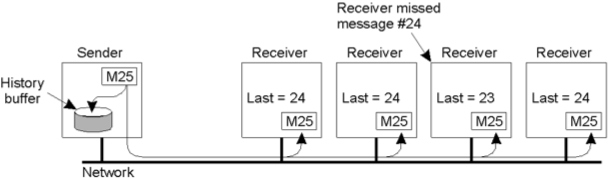
\includegraphics[scale=0.47]{reliable-one-many-communication-1.png}
	\caption{The sender sends a message to all receivers}
	\label{fig:reliable-one-many-communication-1}
\end{figure}

\begin{figure}[h]
	\centering
    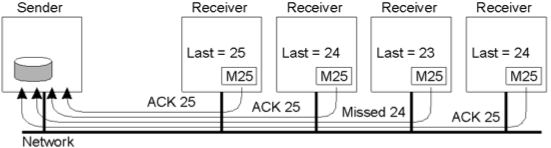
\includegraphics[scale=0.47]{reliable-one-many-communication-2.png}
	\caption{All receivers send an acknowledgement back to the sender}
	\label{fig:reliable-one-many-communication-2}
\end{figure}

\begin{figure}[h]
	\centering
    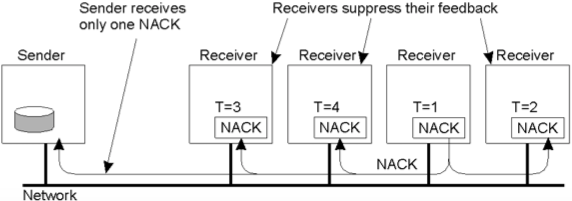
\includegraphics[scale=0.47]{reliable-one-many-communication-3.png}
	\caption{A receiver sends a negative acknowledgement back to the sender}
	\label{fig:reliable-one-many-communication-3}
\end{figure}

\textbf{Question.} What if messages are out of order?

\textbf{Answer.} A NACK-based scheme will not work. We assume in-order message delivery. Otherwise, we have to use an ACK-based scheme.

\textbf{Question.} Instead of sending a bunch of {\ttfamily ACK}s, can a receiver send an {\ttfamily ACK} every $n$th message indicating that it received the last $n$ messages?

\textbf{Answer.} Certainly. This has been tried already. If you have $10000$ nodes, the sender will still get a lot of {\ttfamily ACK}s. If the network is doing its job, a NACK-based scheme will still be more efficient (though the sender will get a lot of {\ttfamily NACK}s if the network is lossy). There are advantages and disadvantages to both schemes based on the properties of the network.

\textbf{Question.} What if the receiver receives a message that it reported as missing at a much later point?

\textbf{Answer.} If we assume in-order message delivery, this will never happen. 

\textbf{Question.} Does this only work across LANs? Or does this also work across the Internet?

\textbf{Answer.} It depends. There is a protocol called \emph{IP multicast} that takes TCP/IP, which is unicast, and extends it to a multicast setting that can be used over WANs. This has not been deployed anywhere because it makes the router stateful. Therefore, while it can be done, there is no real deployment of such a protocol.

\textbf{Question.} Are there protocols other than TCP/IP that provide in-order message delivery?

\textbf{Answer.} While there are many stacks that have been developed, they are not used in place of TCP/IP.

\section{Atomic Multicast}

\textbf{Atomic multicast} guarantees that a message is received by either \emph{all} of the processes or \emph{none} of the processes of a multicast group. In other words, when one process sends a message to a group of processes, either every process or none of the processes receive that message. It should not be possible for some processes to have the message and some processes to not have the message.

\textbf{Problem.} How do we handle when a process in the multicast group crashes?

\textbf{Solution.} We will use a \textbf{group view} where every message is uniquely associated with a group of processes. Each process will have the same view of the group and only send to processes within that group. The basic idea of Figure~\ref{fig:atomic-multicast-example} on how to use a group view to handle a process crashing is below: 
\begin{itemize}
    \item Suppose a process sends a message to every process within a group.
    \item The system must make sure that either \emph{all} or \emph{none} of the processes in the group receive the message.
    \item When a message is sent to every process in the group, there are two possible outcomes:
        \begin{itemize}
            \item If all processes receive that message, the system continues to run without any problems. 
            \item However, if one process does not receive the message as a result of crashing, the system has to stop the message from being delivered to every other process in the group. Most importantly, the process that crashed should then be removed from the group.
        \end{itemize}
\end{itemize}

\textbf{Example.} Atomic multicast can be useful in replicated databases. Suppose we have $3$ replicas of a database. When an update is sent to each replica, we want to guarantee that all or none of the replicas of the database receive the update. If one of the replicas were to not receive the update unlike the other replicas, the database would be left in an inconsistent state. Atomicity is therefore critical to replicated databases.

\begin{figure}[h]
	\centering
    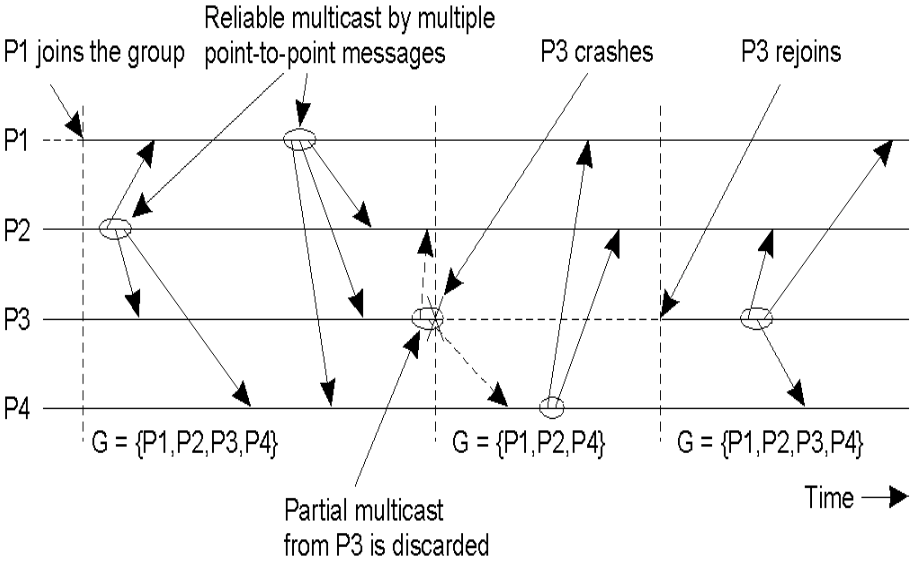
\includegraphics[scale=0.3]{atomic-multicast-example.png}
	\caption{An example of atomic multicast for a group of processes}
	\label{fig:atomic-multicast-example}
\end{figure}

\textbf{Note that the slides \emph{Implementing Virtual Synchrony in Isis} (Slide 17) and \emph{Implementing Virtual Synchrony} (Slide 18) were skipped during the lecture.}

\section{Distributed Commit}

Atomic multicast is an example of a more general problem. In a \textbf{distributed commit}, every process in a group either performs or does not perform a given operation. An operation can range from appending to a log file, delivering a message to a multicast group, or updating a database. We discuss two variations of a distributed commit involving a different number of phases below.

\subsection{Two Phase Commit}

In a \textbf{two phase commit}, there is a \emph{coordinator} that coordinates an operation within a group of \emph{subordinates}. To reiterate, for a given operation, either all or none of the subordinates perform that operation. Note that the node that is a coordinator is also a subordinate. The phases of a two phase commit are as follows:
\begin{itemize}
    \item \textbf{Voting Phase:} All subordinates vote on whether to commit or abort the operation
    \item \textbf{Decision Phase:} All subordinates commit or abort the operation given the results of the voting phase
\end{itemize}
In general, a two phase commit can be broken down into a series of steps:
\begin{enumerate}
    \item The coordinator asks every subordinate to vote on whether to commit or abort a given operation.
    \item Each subordinate sends its vote back to the coordinator:
        \begin{enumerate}
            \item If a subordinate sends a commit vote, it waits for the results of voting from the coordinator.
            \item However, if a subordinate sends an abort vote, it just aborts that operation. This is because the subordinate knows that all other subordinates must abort the operation as well.
        \end{enumerate}
    \item The coordinator gradually collects each vote from the subordinates.
    \item The coordinator reports the results of voting back to the subordinates:
        \begin{enumerate}
            \item If there are only commit votes, the coordinator tells the subordinates to commit. 
            \item However, if there is at least one abort vote, the coordinator tells the subordinates to abort. 
        \end{enumerate} 
    \item All subordinates either commit or abort the operation and send an acknowledgement to the coordinator.
\end{enumerate}

\subsubsection{Coordinator Perspective}

We summarize the role of the \emph{coordinator} during a \emph{two phase commit} in Figure~\ref{fig:two-phase-commit-coordinator-diagram} below:
\begin{itemize}
    \item The coordinator waits for a {\ttfamily Commit} message in the {\ttfamily INIT} state. 
    \item The coordinator sends a {\ttfamily Vote-request} message to the subordinates. 
    \item In the {\ttfamily WAIT} state, the coordinator waits for the subordinates to respond to the {\ttfamily Vote-request} message.
    \item Depending on the responses from the subordinates, the coordinator can do one of two things:
        \begin{itemize}
            \item If the coordinator receives at least one {\ttfamily Vote-abort} message, it issues a {\ttfamily Global-abort} message to the subordinates and then moves to the {\ttfamily ABORT} state.
            \item However, if the coordinator receives only {\ttfamily Vote-commit} messages, it issues a {\ttfamily Global-commit} message to the subordinates and then moves to the {\ttfamily COMMIT} state.
        \end{itemize} 
\end{itemize}

\subsubsection{Subordinate Perspective}

We summarize the role of a \emph{subordinate} during a \emph{two phase commit} in Figure~\ref{fig:two-phase-commit-subordinate-diagram} below:
\begin{itemize}
    \item In the {\ttfamily INIT} state, a subordinate waits for a {\ttfamily Vote-request} message from the coordinator.
    \item Upon receiving a {\ttfamily Vote-request} message from the coordinator, the subordinate either sends a {\ttfamily Vote-commit} message or a {\ttfamily Vote-abort} message back to the coordinator depending on if it can perform the operation:
        \begin{itemize}
            \item If the subordinate replies with a {\ttfamily Vote-commit} message, it moves to the {\ttfamily READY} state.
            \item However, if the subordinate replies with a {\ttfamily Vote-abort} message, it moves to the {\ttfamily ABORT} state. This is because the subordinate knows that all other subordinates must abort as well.
        \end{itemize}
    \item Once the subordinate is in the {\ttfamily READY} state, it waits for a {\ttfamily Global-abort} message or a {\ttfamily Global-commit} message that moves it to the {\ttfamily ABORT} state or the {\ttfamily COMMIT} state respectively. 
\end{itemize}

\begin{figure}[h]
    \centering
    \begin{subfigure}{.5\textwidth}
        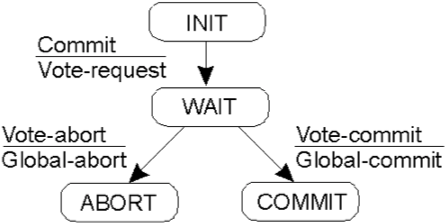
\includegraphics[width=\textwidth]{two-phase-commit-coordinator-diagram.png}
    	\caption{The role of the coordinator}
    	\label{fig:two-phase-commit-coordinator-diagram}
    \end{subfigure}%
    \begin{subfigure}{.5\textwidth}
        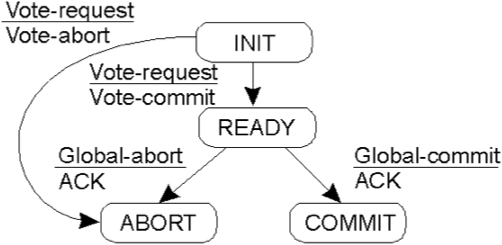
\includegraphics[width=\textwidth]{two-phase-commit-subordinate-diagram.png}
    	\caption{The role of a subordinate}
    	\label{fig:two-phase-commit-subordinate-diagram}
    \end{subfigure}
    \caption{The flow of a two phase commit}
\end{figure}

\subsubsection{Crash Failure Recovery}

We discuss two kinds of crash failures that can occur during a two phase commit below.

\textbf{Subordinate Crash Failure.} \emph{How do we handle when a subordinate crashes?} Suppose that a subordinate crashes during a two phase commit. When the subordinate recovers, it will be in one of the following states:
\begin{itemize}
    \item {\ttfamily INIT}: If the subordinate recovers in the {\ttfamily INIT} state, it has not voted yet. As a result, the coordinator will still be waiting for a vote from the subordinate. Therefore, the coordinator should tell all other subordinates to abort. When the subordinate finally comes back up, it will see that all other subordinates have aborted and then abort as well. Another way to do this is to just have the subordinate send an abort vote when it finally comes back up.
    \item {\ttfamily ABORT}: If the subordinate recovers in the {\ttfamily ABORT} state, it has aborted the operation already. The coordinator would have then already issued an abort to all other subordinates given the abort vote of this subordinate. Therefore, the subordinate can stay in this state or move to the {\ttfamily INIT} state.
    \item {\ttfamily COMMIT}: If the subordinate recovers in the {\ttfamily COMMIT} state, it has committed the operation already. The coordinate would have then already issued a commit to all other subordinates given the commit vote of this subordinate. Therefore, the subordinate can stay in this state or move to the {\ttfamily INIT} state.
    \item {\ttfamily READY}: If the subordinate recovers in the {\ttfamily READY} state, it has sent a commit vote to the coordinator already. However, once the coordinator receives every other vote, it will either issue an abort or a commit to all other subordinates depending on the results of the vote. When the subordinate finally recovers, it will not know what to do. It must therefore ask a neighbor for the results of the vote.
\end{itemize}

\textbf{Coordinator Crash Failure.} \emph{How do we handle when the coordinator crashes?} This is where a two phase commit has some trouble. If the coordinator fails during the voting phase, every subordinate can either get stuck in deadlock or be inconsistent. For instance, suppose that the coordinator calls for a vote. The subordinates in turn vote to commit the operation and then move to the {\ttfamily READY} state. Unfortunately, however, the coordinator receives every vote but crashes before sending the results of the vote to the subordinates. 

\emph{Can the subordinates determine what to do?} Nah, here are some options that all run into problems:
\begin{itemize}
    \item \textbf{The subordinates can ask each other if they voted to commit or abort the transaction.} This is unsafe because the node that is a coordinator is also a subordinate. Suppose that all subordinates agree to commit the transaction. If the coordinator had decided to abort the transaction, the system will transition to an inconsistent state where every subordinate commits the transaction even though the coordinator had aborted the transaction.
    \item \textbf{The subordinates can abort the transaction.} This is unsafe because the node that is a coordinator is yet again also a subordinate. Suppose that all subordinates originally voted to commit the transaction. The coordinator then committed the transaction but crashed before it could send the outcome of voting to all other subordinates. In this scenario, the coordinator would have committed the transaction while the subordinates would have aborted the transaction.
    \item \textbf{Wait for the coordinator to come back up.} If the coordinator never comes back, the subordinates will be deadlocked. While this preserves the safety property, it does not satisfy the liveness property. 
\end{itemize}

\textbf{Question.} How does this differ from a distributed snapshot?

\textbf{Answer.} A distributed snapshot is a way for all of the nodes to save their state in a consistent way. A distributed commit is a generalization that can be extended to other operations like appending to a log file or updating a database.

\textbf{Question.} Does the approach used by a distributed snapshot work for a distributed commit?

\textbf{Answer.} The big difference between a distributed snapshot and a distributed commit is that we did not assume that there could be node failures in a distributed snapshot. We want a distributed commit to still work in the presence of node failures.

\textbf{Question.} Under what conditions can a subordinate go from the {\ttfamily INIT} state to the {\ttfamily ABORT} state directly?

\textbf{Answer.} This will only happen when the subordinate votes to abort the operation.

\textbf{Question.} Why would a transaction be aborted?

\textbf{Answer.} A transaction can be aborted for any reason. Maybe something went wrong with it. The reason why a transaction has been aborted should not be a concern here. 

\textbf{Question.} Can a vote have an expiration time?

\textbf{Answer.} It could. The problems related to the coordinator do not go away though.

\textbf{Question.} Is the coordinator a single point of failure?

\textbf{Answer.} Yes, we will talk about this with Paxos.

\textbf{Note that the slides \emph{Implementing Two-Phase Commit} (Slide 21) and \emph{Implementing 2PC} (Slide 22) were skipped during the lecture. Moreover, the slide \emph{Recovering from a Crash} was skipped because it was discussed prior to reaching that slide.}

\subsection{Three Phase Commit}

In order to handle coordinator crash failures, a \textbf{three phase commit} adds a \textbf{precommit phase} to the phases of a two phase commit. This involves adding a {\ttfamily PRECOMMIT} state between the {\ttfamily WAIT} state and the {\ttfamily COMMIT} state in the coordinator and between the {\ttfamily READY} state and the {\ttfamily COMMIT} state in a subordinate. We see that everything stays the same aside from a few \hl{highlighted} steps that have been added or modified below.

\subsubsection{Coordinator Perspective}

We summarize the role of a \emph{coordinator} during a \emph{three phase commit} in Figure~\ref{fig:three-phase-commit-subordinate-diagram} below:
\begin{itemize}
    \item The coordinator waits for a {\ttfamily Commit} message in the {\ttfamily INIT} state. 
    \item The coordinator sends a {\ttfamily Vote-request} message to the subordinates. 
    \item In the {\ttfamily WAIT} state, the coordinator waits for the subordinates to respond to the {\ttfamily Vote-request} message.
    \item Depending on the responses from the subordinates, the coordinator can do one of two things:
        \begin{itemize}
            \item If the coordinator receives at least one {\ttfamily Vote-abort} message, it issues a {\ttfamily Global-abort} message to the subordinates and then moves to the {\ttfamily ABORT} state.
            \item \hl{However, if the coordinator receives only {\ttfamily Vote-commit} messages, it issues a {\ttfamily Prepare-commit} message to the subordinates and then moves to the {\ttfamily PRECOMMIT} state.}
        \end{itemize} 
    \item \hl{Once the coordinator receives a {\ttfamily Ready-commit} message from the subordinates, it issues a {\ttfamily Global-commit} message  to the subordinates and then moves to the {\ttfamily COMMIT} state.}
\end{itemize}

\subsubsection{Subordinate Perspective}

We summarize the role of a \emph{subordinate} during a \emph{three phase commit} in Figure~\ref{fig:three-phase-commit-subordinate-diagram} below:
\begin{itemize}
    \item In the {\ttfamily INIT} state, a subordinate waits for a {\ttfamily Vote-request} message from the coordinator.
    \item Upon receiving a {\ttfamily Vote-request} message from the coordinator, the subordinate either sends a {\ttfamily Vote-commit} message or a {\ttfamily Vote-abort} message back to the coordinator depending on if it can perform the operation:
        \begin{itemize}
            \item If the subordinate replies with a {\ttfamily Vote-commit} message, it moves to the {\ttfamily READY} state.
            \item However, if the subordinate replies with a {\ttfamily Vote-abort} message, it moves to the {\ttfamily ABORT} state. This is because the subordinate knows that all other subordinates must abort as well.
        \end{itemize}
    \item \hl{Once the subordinate is in the {\ttfamily READY} state, it waits for a {\ttfamily Global-abort} message or a {\ttfamily Prepare-commit} message that moves it to the {\ttfamily ABORT} state or the {\ttfamily PRECOMMIT} state respectively.}
    \item \hl{The subordinate waits in the {\ttfamily PRECOMMIT} state until receiving a {\ttfamily Global-commit} message from the coordinator that moves it to the {\ttfamily COMMIT} state.}
\end{itemize}

\begin{figure}[h]
    \centering
    \begin{subfigure}{.5\textwidth}
        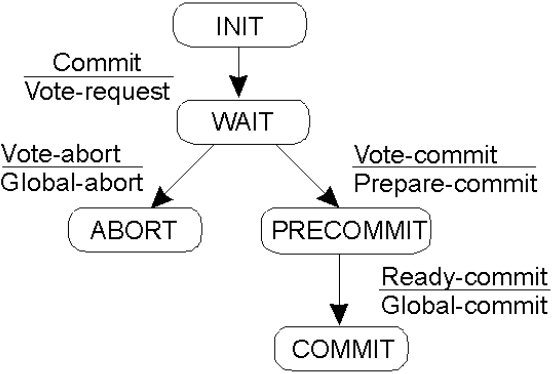
\includegraphics[width=\textwidth]{three-phase-commit-coordinator-diagram.png}
    	\caption{The role of the coordinator}
    	\label{fig:three-phase-commit-coordinator-diagram}
    \end{subfigure}%
    \begin{subfigure}{.5\textwidth}
        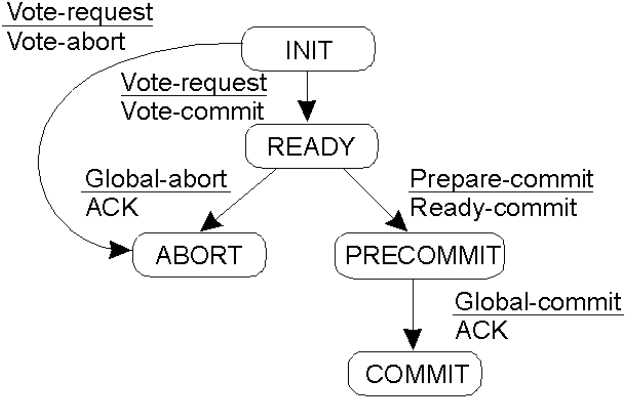
\includegraphics[width=\textwidth]{three-phase-commit-subordinate-diagram.png}
    	\caption{The role of a subordinate}
    	\label{fig:three-phase-commit-subordinate-diagram}
    \end{subfigure}
    \caption{The flow of a three phase commit}
\end{figure}

\subsubsection{Crash Failure Recovery}

\textbf{How does this handle coordinator crash failures?} Suppose that the coordinator asks for a vote and then receives a vote from every subordinate. This means that all subordinates have moved to the {\ttfamily READY} state. Now let us assume that the coordinator crashes and so the subordinates never receive the results of voting from the coordinator. In this scenario, it would be safe for the subordinates to abort the operation. If the coordinator were to come back up, it would be in the {\ttfamily PRECOMMIT} state rather than the {\ttfamily COMMIT} state. This means that the coordinator would not have committed the transaction yet. Once the coordinator finally comes back up, the subordinates can tell the coordinator that the transaction has been aborted.

\textbf{Question.} Should there be a transition from the {\ttfamily PRECOMMIT} state to the {\ttfamily ABORT} state?

\textbf{Answer.} Yes. The diagram does not show what happens in the case of failure though.

\section{Replication for Fault Tolerance}

As an aside, replication can be used for two different purposes. It is possible to use replicas of a service for either performance reasons (\textbf{Technique 1}) or fault tolerance reasons (\textbf{Technique 2}). Note that this lecture has mostly focused on replication for fault tolerance.

\textbf{Technique 1:} A request can be split between different replicas of a service
\begin{itemize}
    \item If one replica fails, we can send requests to other replicas.
    \item This is suitable for crash fault tolerance because we can use another replica when one replica crashes.
\end{itemize}

\textbf{Technique 2:} A request can be sent to all replicas of a service
\begin{itemize}
    \item All replicas vote on their results and take the majority result.
    \item This is suitable for Byzantine fault tolerance.
    \item Examples of this technique include 2PC, 3PC, and Paxos.
\end{itemize}

\section{Consensus and Agreement}

\textbf{Agreement vs. Byzantine Agreement vs. Consensus}
\begin{itemize}
    \item \textbf{Agreement}: All processes must agree on the result of some computation or to perform some operation (like a commit, an abort, a leader election, or a database update). If there is a problem with a process, this will not work because there cannot be total agreement.
    \item \textbf{Byzantine Agreement}: A coordinator makes a decision based on the majority vote of every process (i.e., the Byzantine Generals Problem). If there is a problem with the coordinator, this will not work.
    \item \textbf{Consensus}: All processes act as a coordinator and ask all other processes for a majority vote. This is a group decision and does not require a coordinator. Note that there can only be crash faults here.
\end{itemize}

\textbf{Properties of a Consensus Protocol}
\begin{itemize}
    \item \textbf{Agreement}: Every nonfaulty process must \emph{agree} on the same value.
    \item \textbf{Termination}: Every nonfaulty process must \emph{decide} on some value.
    \item \textbf{Validity}: If all processes \emph{propose} a value, all nonfaulty processes must \emph{decide} on that value.
    \item \textbf{Integrity}: 
        \begin{itemize}
            \item Every nonfaulty process \emph{decides} at most one value.
            \item If a nonfaulty process \emph{decides} on a value, a process must have \emph{proposed} that value.
        \end{itemize}
\end{itemize}

\section{2PC/3PC Problems}

Both two phase commits and three phase commits experience problems in the presence of different types of failures. While the \textbf{safety} property can be ensured, the \textbf{liveness} properties cannot always be guaranteed due to node failures and network failurs: the system will never perform an operation that leads to an inconsistent state (satisfying the safety property) but can still be deadlocked (violating the liveness property). We describe a few caveats associated with each type of commit below.

\textbf{Two Phase Commit}
\begin{itemize}
    \item It must wait for the coordinator and the subordinates to be running.
    \item It requires all nodes to vote.
    \item It requires the coordinator to always be running.
\end{itemize}

\textbf{Three Phase Commit}
\begin{itemize}
    \item It can handle coordinator failures.
    \item But network failures are still a problem.
\end{itemize}

There has been an implicit assumption that there could only be node failures instead of network failures during a two or three phase commit. While a node could crash in the network, the network would never experience any issues. Suppose, however, that the network was partitioned into two partitions due to some problem. Although both partitions will continue to function correctly, each partition cannot communicate with each other. \textbf{By definition, if the network is partitioned due to some problem, a two or three phase commit cannot work because every node is required to vote on the answer.}

In order to eliminate such an assumption, we have to revisit the definition of \emph{agreement}. Rather than requiring the vote of every node, we can just require the vote of the majority of nodes. Therefore, if the network were to be separated into two partitions, the partition with the majority of nodes can still continue to function properly. This idea forms the basis of \textbf{Paxos}, a consensus protocol. \textbf{Instead of requiring every node to vote, Paxos only requires the majority of nodes to vote.}

\section{Paxos Requirements}

Paxos satisfies the following properties:
\begin{itemize}
    \item Safety (\emph{Correctness})
        \begin{itemize}
            \item All nodes must agree on the same value.
            \item The agreed upon value must be computed by some node.
        \end{itemize}
    \item Liveness (\emph{Fault Tolerance})
        \begin{itemize}
            \item If less than $\frac{n}{2}$ nodes fail, the remaining nodes will eventually reach agreement. This allows the system to make progress in the presence of failures.
            \item Note that that liveness is not guaranteed if there is a steady stream of failures as the protocol determines what to do. If a node fails in the middle of the protocol, it must be restarted.
        \end{itemize}
    \item \textbf{Why is agreement hard?} Because even in the face of failures, we still need to reach agreement.
        \begin{itemize}
            \item The network might be partitioned. 
            \item The leader may crash during solicitation or before
            announcing the outcome of voting. While the current round will not produce any results, a new leader will be elected through leader election. All nodes will then vote again. 
            \item A new leader may propose different values from the value that had been agreed upon originally.
            \item Several nodes may become a leader at the same time. This is possible when the network is partitioned due to a network failure. The left half will elect a new leader while the right half will have the old leader, and they will still continue to function properly. Both sides of the partition may agree on different things unfortunately.
        \end{itemize}
\end{itemize}

\section{Paxos Introduction}

Paxos is a $3$ phase protocol. Similar to the other approaches that have been discussed, we have a leader. The leader proposes a solution to some computation to every node in the system. Rather than asking the nodes whether or not the transaction should be committed or aborted, we instead ask the nodes whether they agree or disagree with the proposed solution. If the majority of nodes agree with the answer, the leader will determine that the answer is correct. However, if the majority of the nodes disagree with the answer, we repeat this process. Each node can also propose its own solution (though this was not discussed in detail). As a side note, the leader only has to wait for the majority of nodes to vote instead of all of the nodes.

\textbf{Note that the majority of the slides on Paxos were skipped and saved for the next lecture.}
 
\end{document}